
In multi-agent systems there are different ways the agents can be organized. 
Depending on the architecture of this organization the system will adapt to 
the given problem in different ways depending on the architecture. 

When agents work in teams, each team has its function. When a team reaches a goal, it will share this information with the other teams.
\begin{figure}[ht]
    \centering
    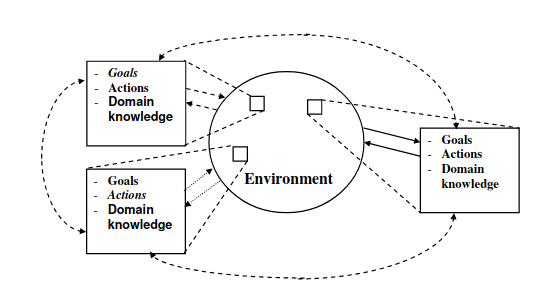
\includegraphics[scale=0.6]{teamcommunication.png}
    \caption[Communication as teams]{Communication as teams}
\end{figure}

For example a patrol, search, and track problem. Where each team has its own goal. 
Team A will patrol an area and report if it finds some abnormalities. Team B will search for these abnormalities in the area and report any findings to team C. 
Team C will then on its turn start and track these objects.

Coalitions, like teams, consist of multiple UAVS working together. In coalitions not each UAV has the same goal. 
The agents will adapt to the information and the environment to change their goal.

\newpage

\begin{figure}[ht]
    \centering
    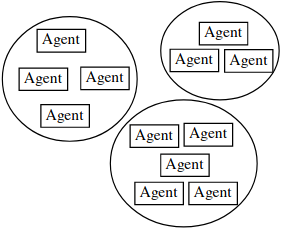
\includegraphics[scale=0.6]{coalitions.png}
    \caption[Communication as coalitions]{Communication as coalitions}
\end{figure}
Let’s take the same example from teams. Each coalition will take on a subarea of the original area. Within the coalition, 
each agent will take action depending on the current state of the area ( if an object is found or not ). 
Depending on the information an agent can decide to switch actions, for example from searching to tracking.

In a hologenic hierarchy all the agents will communicate with each other, prioritizing the one closest to them. 
Each UAV will share its current state and other agents will adapt to this information. When receiving new information 
from the blackboard system, agent states can change, updating the entire hierarchy. 

\begin{figure}[ht]
    \centering
    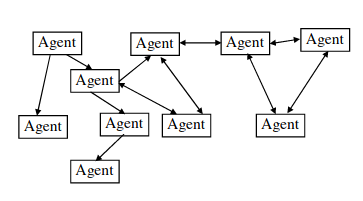
\includegraphics[scale=0.6]{agentComsClosest.png}
    \caption[Communication as hologenic hierarchy]{Communication as hologenic hierarchy}
\end{figure}